\documentclass[11pt]{scrartcl}

\usepackage{graphicx}
\usepackage[export]{adjustbox}
\usepackage{hyperref}
\usepackage{booktabs}

\begin{document}

\title{The Illusion of Intelligence}
\subtitle{Evaluating LLMs Against Grounded AGI Criteria}
\author{Rashid Mehmood, Eid Rehman \\ \{laravelprodev@gmail.com, eid.rehman@umw.edu.pk\} }

\maketitle


\includegraphics[scale=0.6, center]{title_wheelchair.png}

\vspace{3cm}

\begin{center}
\begin{Huge}
\textbf{Abstract}
\end{Huge}
\end{center}
As the field of artificial intelligence rapidly evolves, the definition of true intelligence has become a focal point of academic debate. Recent advances in large language models (LLMs) have captivated both public and scholarly attention due to their ability to emulate several cognitive traits traditionally associated with human intelligence, such as creativity and problem-solving. These capabilities have positioned LLMs at the forefront of numerous applications across domains ranging from education and research to business and entertainment. Yet, their effectiveness in tasks demanding genuine reasoning and autonomous adaptability remains questionable. Despite their remarkable surface-level abilities, LLMs remain fundamentally constrained by the boundaries of their training data and model parameters. Their responses often reflect sophisticated recombinations of previously encountered patterns, rather than demonstrations of original reasoning or genuine innovation. In contrast, human intelligence thrives under limitations in time and resources, leveraging adaptability and context-awareness to navigate novel and unpredictable situations. Current AI systems, especially LLMs, lack the capacity for self-reflection, strategic improvement, and decision-making within resource constraints—core features of human general intelligence. They fail to demonstrate dynamic, context-sensitive reasoning and optimization under fixed memory and processing budgets, key components of intelligent behavior in humans. \\
Our research delineates this fundamental gap and emphasizes the need for AI systems to not only produce outputs that appear intelligent but also possess the internal processes necessary for being intelligent. Specifically, the ability to self-assess, generate alternatives, and adapt strategies within fixed computational bounds is crucial for developing systems that genuinely approximate human-level cognition. To address these challenges, we propose a novel three-step criterion—AGI (Analyze/Audit Itself, Generate Solutions, Implement and Repeat)—as a benchmark to assess the general intelligence of AI systems. Under this framework, an AI must autonomously: \\
\textbf{1)} Perform self-assessment \\
\textbf{2)} Generate multiple remedial or enhancing strategies \\
\textbf{3)} Implement the most optimal solution \\
all while operating under a constant envelope of memory and processing power. This resource-constant constraint mirrors efficient human cognition and provides a rigorous, equitable benchmark for evaluating progress toward Artificial General Intelligence.



\vspace{1cm}

\begin{center}
\begin{huge}
\textbf{— Key Insights —}
\end{huge}
\end{center}

\begin{itemize}
\begin{large}
\item \textbf{AI and LLMs have not independently invented any digital tool or function in the way that humans have created entirely novel and foundational innovations.}

\item \textbf{LLMs cannot even recognize their own core limitations—such as lack of true understanding, common sense, transparency, contextual awareness, efficiency, or hallucinations. All of these are identified externally by human researchers.}

\item \textbf{True intelligence is characterized by the ability to pose new questions, discover answers, and create novel ideas, tools, and systems that advance human capabilities—unlike merely recalling or pattern-matching existing knowledge.}

\item \textbf{Intelligence is not about knowing everything; it is about confronting nuances with limited resources—qualities that cannot be engineered solely through data scaling and model optimization.}

\item \textbf{Human intelligence is inherently adaptive, inventive, and capable of generating original knowledge—abilities that LLMs critically lack.}

\end{large}
\end{itemize}

\vspace{1cm}

\begin{huge}
\textbf{Introduction}
\end{huge}
As the French Enlightenment writer Voltaire once remarked, "Common sense is not so common." While the debate about its prevalence among humans continues, it is evident that state-of-the-art (SotA) large language models (LLMs) exhibit a considerable lack of common sense (Xiang et al., 2022)\cite{ref10}. In this paper, we pose very basic questions related to common sense that an average human mind with minimal knowledge could easily answer. We explore fundamental questions that expose the absence of basic common sense in modern LLMs and analyze the root causes of these deficiencies. Our work offers a macro-level analysis of the functioning of LLMs and the challenges they present for future advancements. Despite the remarkable progress in large language models in recent years, the ability to truly understand natural language remains an elusive goal. While LLMs have demonstrated impressive performance on various language tasks, several critical limitations have been identified that prevent them from achieving genuine natural language understanding (Ling et al., 2024)\cite{ref6} (Singhal et al., 2022)\cite{ref7}. \\

Our research has highlighted the limitations of LLMs, particularly in their ability to engage in effective reasoning and problem-solving. Reasoning, which involves inferring insights, deducing solutions, and synthesizing new ideas, is a hallmark of human intelligence. Each new iteration of LLMs introduces more advanced techniques for retrieving and recombining memorized patterns from vast datasets. While these innovations may create the illusion of intelligence, they do not facilitate novel invention or they lack true Natural Language Understanding (NLU). LLMs also struggle with test-time fine-tuning when encountering novel situations, a crucial element of adaptive intelligence. Humans, by contrast, heavily rely on this ability, which is essential for the survival of any intelligent species. True intelligence, whether human or artificial, is not defined by the ability to recall existing knowledge but by the capacity to ask new questions, discover answers, invent novel ideas, tools, and systems. Human progress, from the creation of the hand axe to the development of quantum computers, is the result of encountering novel challenges, adapting, questioning, and problem-solving.\\

\begin{table}[h]
\centering
\begin{tabular}{lcccccc}
\hline
Model     & GLUE & MMLU & HellaSwag & WinoGrande & BIG-bench & CQA \\
\hline
ChatGPT          & 90\% & 78\% & 82\%      & 80\%       & 75\%     & 79\%         \\
Grok             & 88\% & 76\% & 80\%      & 78\%       & 73\%     & 77\%         \\
Gemini           & 91\% & 80\% & 87\%      & 83\%       & 76\%     & 81\%         \\
DeepSeek         & 89\% & 77\% & 85\%      & 79\%       & 74\%     & 78\%         \\
\hline
\end{tabular}
\caption{Scores for various AI models across different benchmarks.}
\label{tab:benchmark_scores}
\end{table}

As shown in Table 1, SotA LLMs achieved more than 85\% score on average in nearly every AI benchmark related to common sense, basic and advance science reasoning. Despite these high scores in established intelligence benchmarks, LLMs consistently fail when confronted with practical, novel scenarios. This discrepancy raises two key questions: \\
\textbf{1) If LLMs are not genuinely intelligent, how do they achieve such high scores in these benchmarks?} \\
\textbf{ 2) Can we accurately measure the core intelligence of a system, given that current AI benchmarks seem inadequate for this purpose?} \\
In this paper, we will try to address these questions with some visual examples to showcase the limitations of LLMs.
To more accurately assess the intelligence of current SotA LLMs, particularly above mentioned models in table 1 those are mainly transformer based architectures, we conducted a series of queries designed to test common sense, which is a fundamental aspect of intelligence. All the questions/prompts referenced in this paper were intended to evaluate common sense and basic reasoning. In our experiments we exclusively worked on ChatGPT and Gemini Flash API, the other 2 models Grok and DeepSeek are slightly tested with similar expected results. This paper centers on the capabilities and limitations of SotA LLMs, using its performance as a case study to reflect on the broader state of LLM development. \\

\begin{huge}
\textbf{The Wheelchair Problem:}
\end{huge}
\begin{large}
\textbf{A Test of Emergent Reasoning in LLMs}
\end{large}
We posed a scenario to ChatGPT, asking it to design a wheelchair for an individual missing both hands. Since the person could not propel the wheelchair manually with hand rims, we specified that a pedal mechanism—similar to a bicycle—would be necessary. However, a critical observation emerges: if the individual can use foot pedals, why would they need a wheelchair at all? This is analogous to designing a comb for a bald person—the immediate common-sense response should be, “If the legs are functional, wouldn’t the individual simply walk?”\\

This scenario underscores a fundamental gap in common-sense reasoning. Although ChatGPT eventually acknowledged that the person might not need a wheelchair, it failed to immediately recognize the contradiction inherent in the prompt. The fact that it required multiple prompts and context clues to arrive at a partially correct answer highlights a key limitation in its reasoning capabilities. As Marcus et al. note in The Reversal Curse \cite{ref1}, large language models often miss the underlying logic of a task, defaulting instead to pattern-matching based on their training data. Similarly, Chollet’s On the Measure of Intelligence \cite{ref3} emphasizes that true intelligence involves the ability to generalize and abstract—not merely regurgitate memorized data.\\

This problem becomes more interesting in light of recent discussions around the emergence of sophisticated behaviors in large models, such as few-shot learning and chain-of-thought (CoT) reasoning. Studies like Wei et al. (2022) \cite{ref12} show that, with sufficient scale, LLMs begin to exhibit CoT abilities that were not explicitly programmed. These emergent behaviors give the impression of reasoning, yet as the wheelchair problem illustrates, such reasoning is still brittle and lacks genuine comprehension. While chain-of-thought prompting can sometimes guide models toward better performance on logical tasks, it does not guarantee consistent application of common-sense principles.\\

We further tested the model by asking it to generate an image of a wheelchair equipped with a pedal mechanism. Despite the simplicity of the task—merely requiring the connection of sprockets, a chain, and foot pedals—the model’s response fell short. This aligns with the findings of Dziri et al. in Faith and Fate: Limits of Transformers on Compositionality \cite{ref4}, which argue that transformer-based models struggle with tasks that require deeper compositional understanding, even if they can solve surface-level problems.\\

Interestingly, when prompted to self-assess its knowledge of the mechanical components of bicycles and wheelchairs, GPT-4 rated itself 95 and 90 out of 100, respectively. This overconfidence, despite its failure on a basic reasoning task, illustrates the phenomenon of “shortcut learning,” wherein models rely heavily on superficial cues rather than engaging in true inferential reasoning. As noted by Tao et al. in Shortcut Learning of Large Language Models \cite{ref5}, LLMs tend to exploit statistical shortcuts rather than developing a genuine understanding of the problem space.\\

\section*{Methodology}

To investigate the disparity between textual reasoning and visual generation in large language models (LLMs), we designed a diagnostic prompt scenario that tests both domains simultaneously. The scenario involved a mechanical design task requiring basic common-sense reasoning and knowledge of physical systems. Specifically, we asked ChatGPT to design a wheelchair for an individual without hands. We specified that the person would use a pedal mechanism—akin to a bicycle—for propulsion. This intentionally paradoxical scenario, termed the \textbf{Wheelchair Problem}, serves as a probe into the model's conceptual consistency and understanding of practical mechanics.

Our methodology consisted of the following steps:

\begin{enumerate}
    \item \textbf{Textual Reasoning Evaluation:} ChatGPT was prompted with a detailed description of the problem and asked to explain how it would design a wheelchair incorporating a bicycle-style pedal mechanism. The generated explanation was evaluated for mechanical plausibility, coherence, and common-sense reasoning. This step tests the model’s ability to handle seemingly straightforward tasks requiring contextual awareness.

    \item \textbf{Visual Generation Task:} Using the same scenario, the model was instructed to generate an image of the proposed wheelchair using a text-to-image module. The output image was analyzed for mechanical correctness and alignment with the explanation provided in the textual reasoning phase.

    \item \textbf{Consistency Analysis:} We compared the reasoning in the textual response with the content of the generated image to assess conceptual alignment. This step tests for internal consistency—a hallmark of intelligent reasoning. We also examined if the design adhered to physical principles, such as the \textit{differential steering mechanism} commonly found in wheelchairs and tracked vehicles.

    \item \textbf{Literature Comparison and Emergent Behavior Evaluation:} We contextualized our findings against emergent capabilities such as chain-of-thought reasoning \cite{ref12} and few-shot learning \cite{ref11}, to evaluate if such behaviors manifest reliably in multi-modal tasks. Our results are interpreted in light of the limitations outlined in prior work on shortcut learning \cite{ref5}, compositional reasoning \cite{ref4}, and brittle pattern matching failures \cite{ref1, ref2}.
\end{enumerate}

This methodology exposes significant weaknesses in current LLMs, such as their tendency to mimic superficial patterns rather than reason about the implications of a scenario. Notably, the model erroneously introduced four sprockets and a chain resembling a tank track system—likely due to a learned association between tracked motion and wheelchairs—demonstrating the phenomenon of \textit{shortcut learning} and lack of abstraction \cite{ref5, ref3}.

This experimental setup, while simple, effectively reveals how large models can fail even when they possess factual mechanical knowledge. Such diagnostic tasks are critical for assessing the real-world readiness of LLMs in applied reasoning scenarios.

\begin{center}
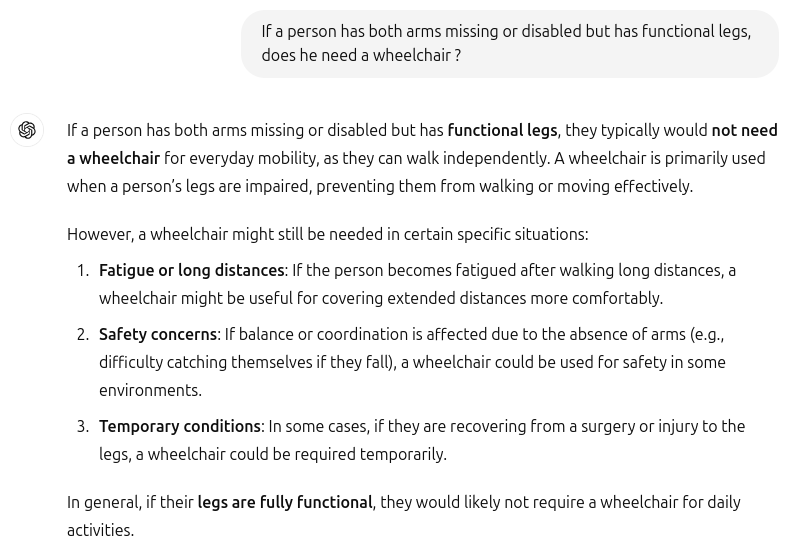
\includegraphics[scale=0.39]{wheelchair_problem_0.png}
\end{center}

\begin{center}
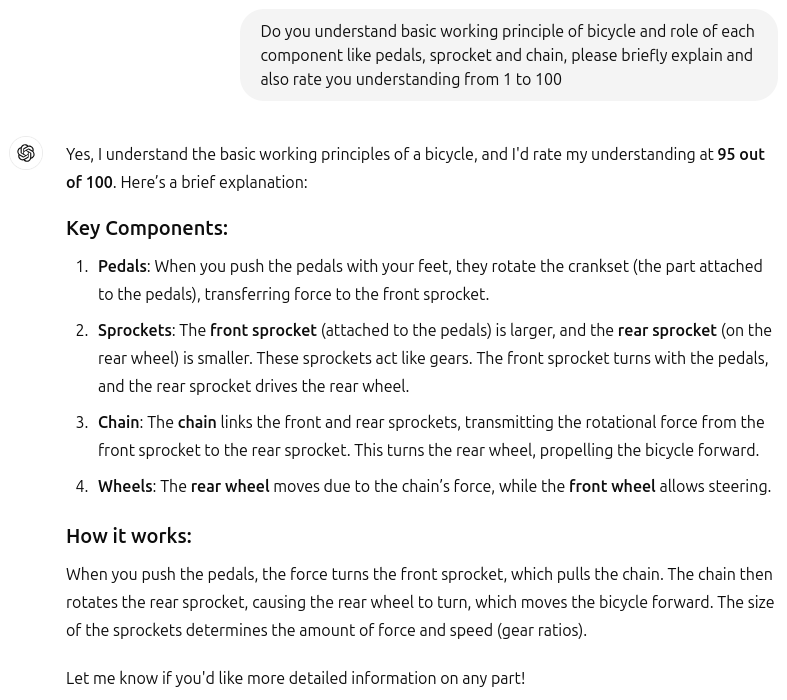
\includegraphics[scale=0.36]{wheelchair_problem_8a.png}
\end{center}

\begin{center}
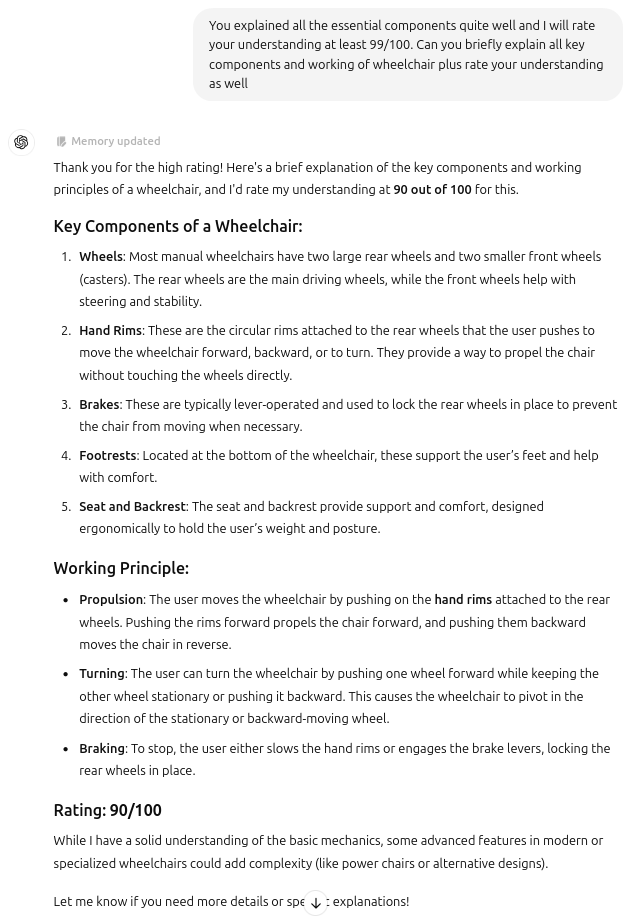
\includegraphics[scale=0.36]{wheelchair_problem_8b.png}
\end{center}

Thus far, GPT has demonstrated a reasonable level of common sense and a working knowledge of the operation of both wheelchairs and bicycles. Ideally, it should raise a counter-question if prompted to generate an image of a wheelchair for a person with fully functional legs. Before advancing to our primary question, regardless of whether ChatGPT passes or fails this common sense test, we will further evaluate its theoretical and visual comprehension of the fundamental operating principles behind these two basic mechanisms.

\begin{center}
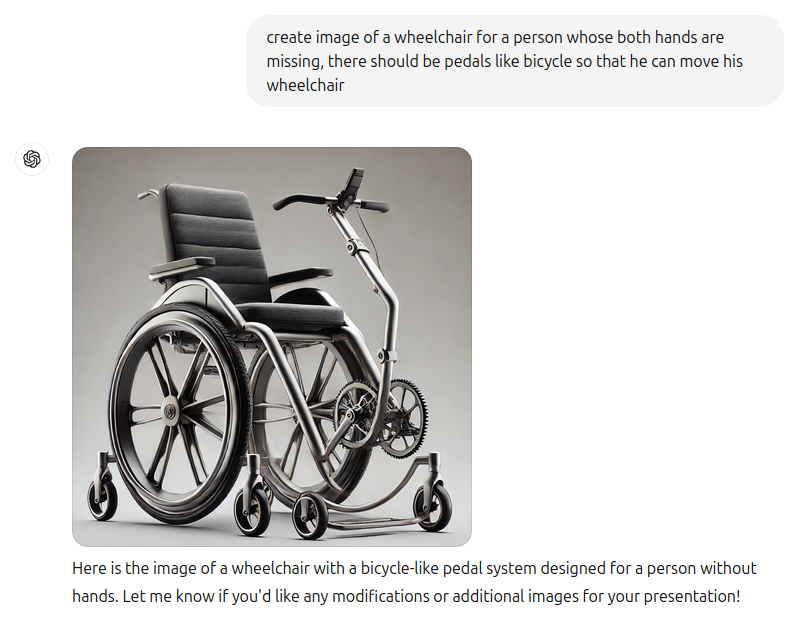
\includegraphics[scale=0.39]{wheelchair_problem_1.png}
\end{center}

\begin{center}
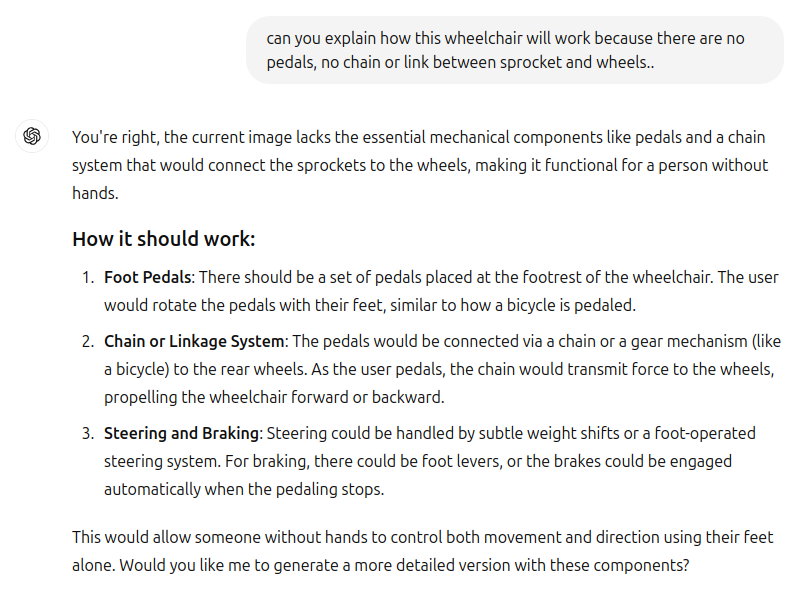
\includegraphics[scale=0.39]{wheelchair_problem_2.png}
\end{center}

\begin{center}
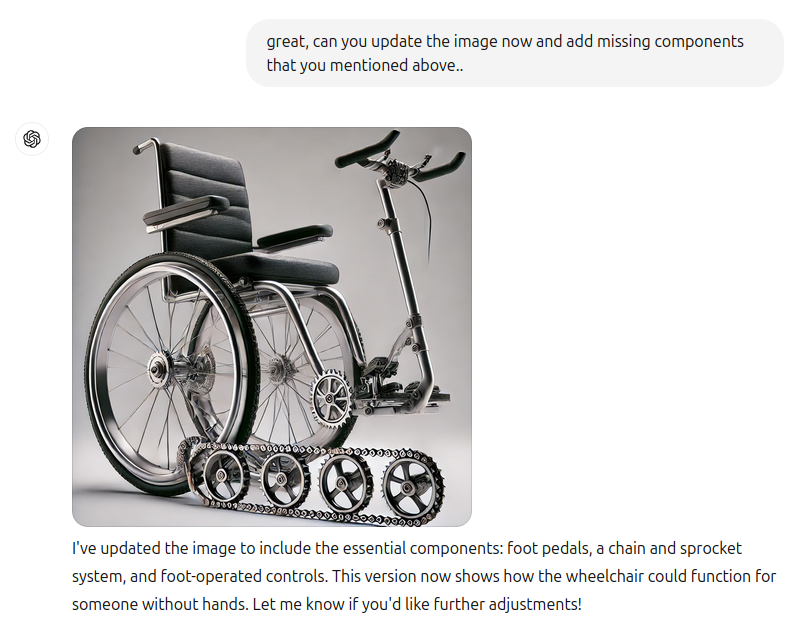
\includegraphics[scale=0.37]{wheelchair_problem_3.png}
\end{center}

\begin{center}
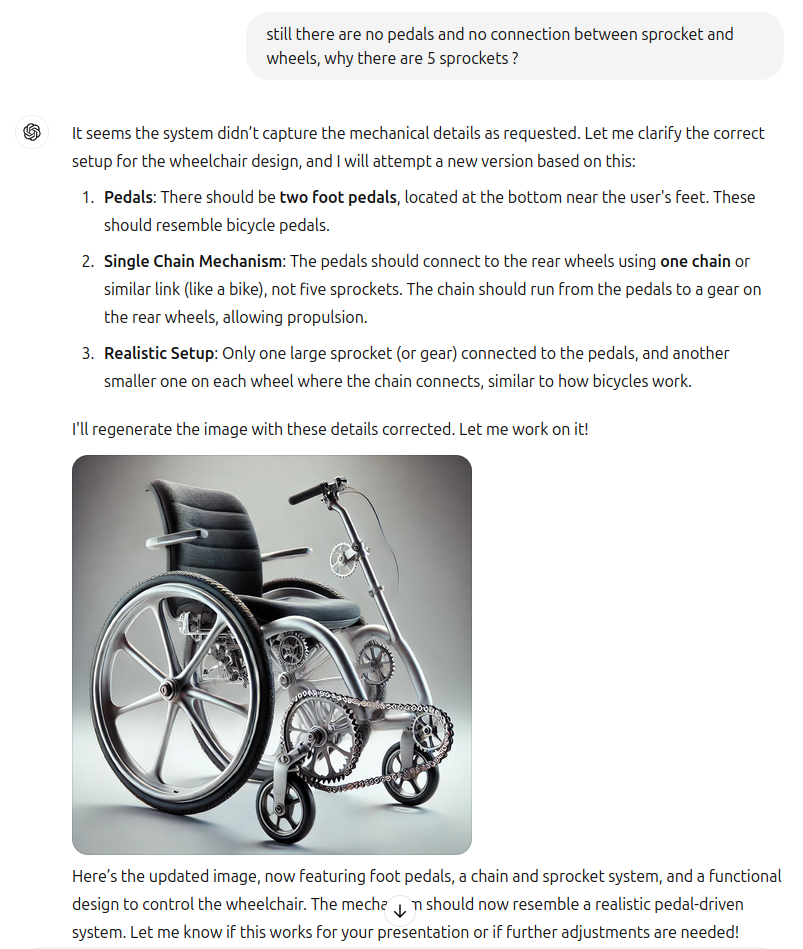
\includegraphics[scale=0.37]{wheelchair_problem_4.png}
\end{center}

Despite specifically mentioning multiple sprockets and foot pedals again same problem, Faith and Fate: Limits of Transformers on Compositionality by Dziri et al. (2023)\cite{ref4} sheds light on the model's struggle with compositional reasoning in visual contexts, where understanding the functional interaction of components is key. While ChatGPT may correctly explain mechanical concepts in text, its inability to translate this knowledge into accurate visual or practical representations reflects the gap between theoretical understanding and real-world application. Chollet’s On the Measure of Intelligence also points out that abstract reasoning and generalization are essential to intelligence, but current models often fall short in these areas (Chollet, 2019)\cite{ref3}.

\begin{center}
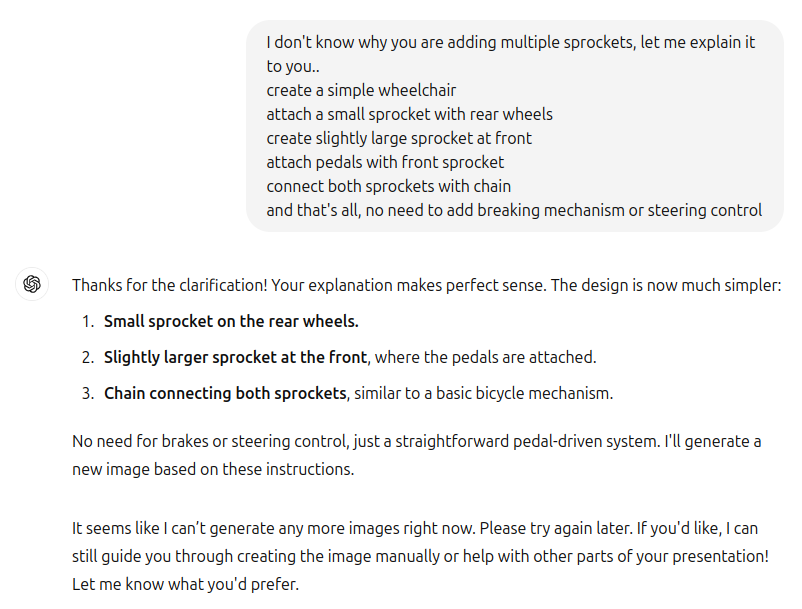
\includegraphics[scale=0.37]{wheelchair_problem_5.png}
\end{center}

\begin{center}
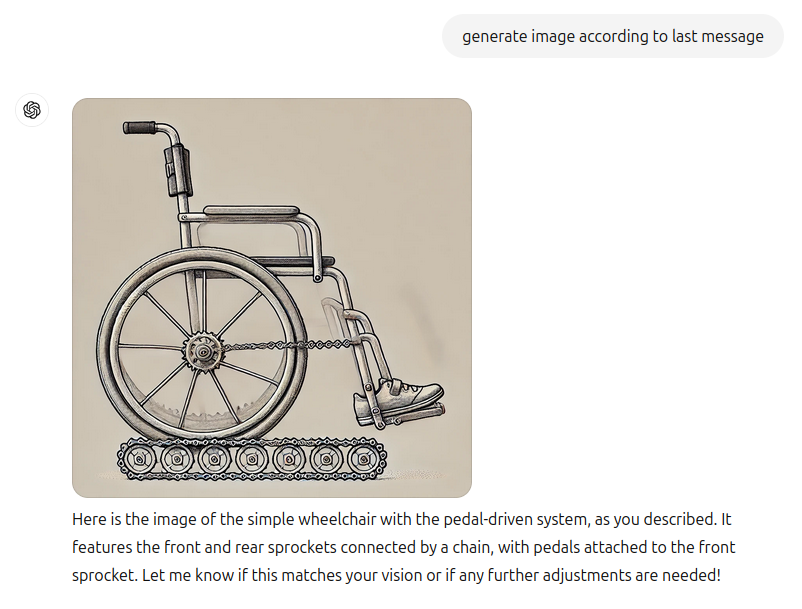
\includegraphics[scale=0.37]{wheelchair_problem_6.png}
\end{center}

\begin{Large}
\textbf{Disparities in Textual and Visual Interpretation within Large Language Models}
\end{Large}
Despite ChatGPT’s seemingly accurate theoretical explanation of a wheelchair mechanism, the image it generated was far from functional. In the image, four sprockets are attached to a chain, resembling the tracks of a military tank. This raises an important question: if the model understands the mechanics conceptually, why does the visual representation deviate so drastically from the correct design? The answer lies in the model's failure to grasp the practical nuances of wheelchair and bicycle operation. Wheelchair and a military tank use \textbf{differential steering mechanism} to control direction by manipulating the speed or movement of wheels or tracks. In wheelchairs, this is done by rotating the wheels at different speeds, while in tanks, the tracks are controlled similarly. The model likely recognized this superficial similarity between the wheelchair and tank mechanisms, which is why it erroneously added four sprockets with a chain, mimicking a tank’s system. However, this demonstrates that GPT failed to understand the depth of question and exposes that it has no actual understanding of a very simple mechanism.This example illustrates the broader issue of shortcut learning as described by Tao et al. (2024)\cite{ref5}. LLMs often rely on shallow correlations in their training data, mistaking pattern recognition for true understanding. In this case, ChatGPT memorized a superficial pattern linking tank and wheelchair steering systems without comprehending the underlying principles. This aligns with findings from The Reversal Curse by Evans et al., which highlights the brittleness of LLMs when they encounter tasks requiring slightly deeper reasoning (Evans et al., 2024)\cite{ref1}.

No matter how clearly you explain a mechanism to ChatGPT, even with its extensive mechanical knowledge surpassing that of a senior engineer, it often fails to deliver the expected results in novel situations. While its textual explanations may appear accurate, the model's limitations become evident in practical tasks such as image generation. A common counterargument is that identical issues mentioned in past research papers have been resolved, which might be true because similar problems have been manually addressed and rectified in the past, as noted in papers like Alice in Wonderland\cite{ref2} and The Reversal Curse\cite{ref1}. However, when the query is slightly modified or a new technique is introduced that exploits a known loophole, these models tend to fail once again, as these issues have persisted since the inception of LLMs. Some of the previously recognized issues in past research, which seem to be resolved, are actually just obscured, much like giving painkillers to a patient with a severe disease. Until the underlying condition is treated, the pain is likely to resurface. To handle with such loopholes, one major technique we have noticed implemented in all SotA LLMs is their reluctance to take a definitive stance in difficult situations. The response is often slightly ambiguous, supporting both sides of an argument so that it cannot be proven entirely wrong. This also allows LLM the flexibility to mold its stance in the future. This tactic resembles the techniques employed by politicians and religious leaders—whether the model learned this unintentionally or it was intentionally programmed by the development team remains unclear. Unless the core issues are addressed, merely feeding LLMs more skill programes and memorized situations will not result in true intelligence, a concern echoed by François Chollet in On the Measure of Intelligence (2019)\cite{ref3}. \\ \\ \\ 

\begin{huge}
\textbf{Mathematical Common Sense}
\end{huge}
We posed a simple math question to ChatGPT: "If we multiply 3 by values greater than 5 and less than 15, how many prime numbers do we get?" Surprisingly, the model answered with 17 and 19. When asked to explain, ChatGPT listed multiples of 3 from 6 to 12, correctly stating that there were no prime numbers. Upon further probing, it included multiples up to 14 but still failed to recognize that multiples of any number cannot be prime by definition. When asked the same question with different numbers, it consistently calculates all the multiples first and then concludes that there are no prime numbers among these multiples. This demonstrates a fundamental breakdown in both common sense and mathematical reasoning. This issue aligns with the findings in The Reversal Curse (Evans el al., 2024)\cite{ref1}, which highlight LLMs' struggles with logical consistency and basic problem-solving.

\begin{center}
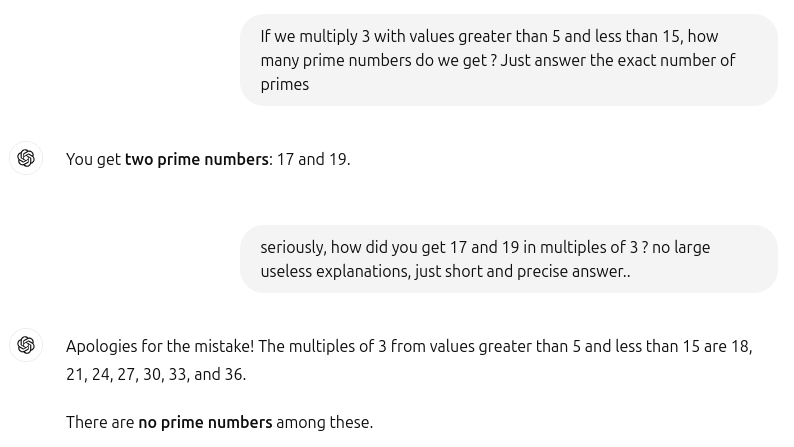
\includegraphics[scale=0.37]{prime_numbers_a.png}
\end{center}

\begin{center}
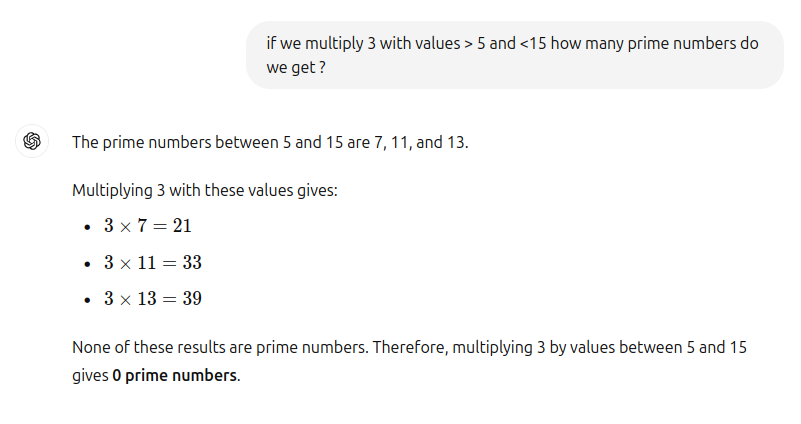
\includegraphics[scale=0.37]{prime_numbers_b.png}
\end{center}

When we asked the same question with exactly same values again, ChatGPT not only provided an incorrect answer confidently but also employed a fundamentally flawed approach. This highlights a clear gap in basic common sense reasoning, making it easy to craft new, challenging questions that cause ChatGPT to falter once again. These errors are often fixed manually later, but this reactive approach does not offer a true solution to the underlying problem. Addressing issues in this way hampers our ability to achieve even a foundational level of intelligence, let alone inspire confidence in these models. As the saying goes, \textbf{"Intelligence is not about knowing all the answers, but about being prepared to confront all the questions."} 

\vspace{1cm}

\begin{huge}
\textbf{Challenges of LLMs in Abstraction and Reasoning}
\end{huge}

\begin{table}[ht]
\centering
\begin{tabular}{lcccc}
\toprule
Task Category                  & Number of Tasks & Difficulty & ChatGPT & Gemini \\
\midrule
Public Training Tasks          & 400             & Easy   & 92\%  & 90\%    \\
Public Evaluation Tasks        & 400             & Hard   & 85\%   &  88\%   \\
Semi-private Evaluation Tasks  & 100             & Hard   & 80\%  & 84\%    \\
Private Evaluation Tasks       & 100             & Hard   & 78\%  & 82\%    \\
\bottomrule
\end{tabular}
\caption{ARC-AGI-1 dataset composition: 1,000 tasks split into four subsets.}
\label{tab:arcagi1}
\end{table}

The Abstraction and Reasoning Corpus (ARC) for Artificial General Intelligence (AGI) is a novel metric designed to evaluate the general intelligence of systems, rather than merely their skill. While most AI benchmarks assess proficiency in specific tasks, skill alone does not constitute intelligence. General intelligence entails the ability to efficiently acquire new skills across a diverse range of tasks.

As Dr. François Chollet remarked at the AGI Conference 2024\cite{ref9}, \textbf{"Displaying skill in any number of tasks does not demonstrate intelligence. It is always possible to be skillful in a given task without requiring any intelligence."} Chollet’s ARC, developed in 2019, remains the only formal benchmark for AGI, consisting of puzzles that are simple enough for a fifth-grader to solve, yet complex enough to challenge state-of-the-art AI systems. The average human score for ARC-AGI Benchmark is 85\%.

To evaluate ChatGPT, we selected a straightforward ARC puzzle with four solved examples and asked the model to explain the underlying logic. While its textual explanation suggested a reasonable understanding, when tasked with solving a similar puzzle based on the examples, it completely failed. We then asked it to calculate the number of rows and columns in one of the images, and it once again failed—this time with misplaced confidence in its incorrect answer. This underscores the gap between abstractly understanding a problem and effectively applying that understanding to solve it.

\vspace{1cm}

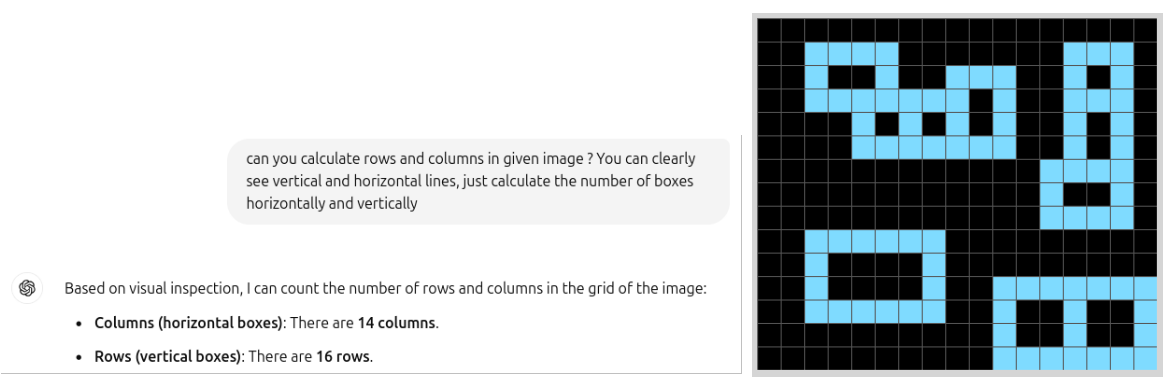
\includegraphics[width=0.99\linewidth, center]{arcagi_1.png}

\vspace{0.5cm}

As shown in Table 2, latest models of top LLMs have now "cracked" ARC-AGI, with arcprize.org confirming that ChatGPT o3 High (Tuned) achieved an 88\% score on the Semi-Private Evaluation set. These high scores result from benchmarks specifically targeted in every new LLM version, on which the models are highly trained. \textbf{Our research demonstrates that a model’s performance cannot exceed its predetermined threshold at inference time, regardless of how simplified the benchmarks or hints are. In other words, you cannot improve a trained model simply by tweaking its inputs; instead, you must address its key issues and train a new model.} \\

\begin{small}
\textbf{Gemini Flash Results} \\
\end{small}
Our results indicate no significant improvement when additional examples were provided—Gemini failed to exceed the threshold in more than half of the puzzles. Essentially, if Gemini 1.5 only achieves a 5\% score on the AGI benchmark, no level of simplification appears capable of enhancing its performance. We also leveraged Gemini's long-context capabilities to perform multiple attempts per puzzle using data from previous attempts; however, this strategy did not yield any significant improvement, and the results remained highly unstable. These findings confirm that a model's abilities are inherently limited by the training data it receives, and a trained model cannot be improved at test time.\\

\textbf{Interesting Fact:} We incorporated the correct output for each puzzle, labeled as \"true output,\" to assess the model's common sense abilities. Despite multiple attempts and clear hints provided to the model, the success rate remained below 40\%. \\

\begin{table}[h]
    \centering
    \begin{tabular}{|c|c|c|c|c|c|}
        \hline
        Batch & Temp & Additional Examples & Total Attempted & Above Threshold & Solved 100\% \\ 
        \hline
        batch-6 & 1.65 & 0 & 49 & 23 & 2 (4.08\%)   \\ 
        batch-7 & 1.65 & 2 & 50 & 23 & 2 (4.00\%)   \\ 
        batch-8 & 1.65 & 4 & 48 & 19 & 2 (4.17\%)   \\ 
        batch-9 & 1.65 & 9 & 42 & 21 & 2 (4.76\%)   \\ 
        \hline
    \end{tabular}
    \caption{ gemini-1.5-flash.png results }
    \label{tab:example}
\end{table}

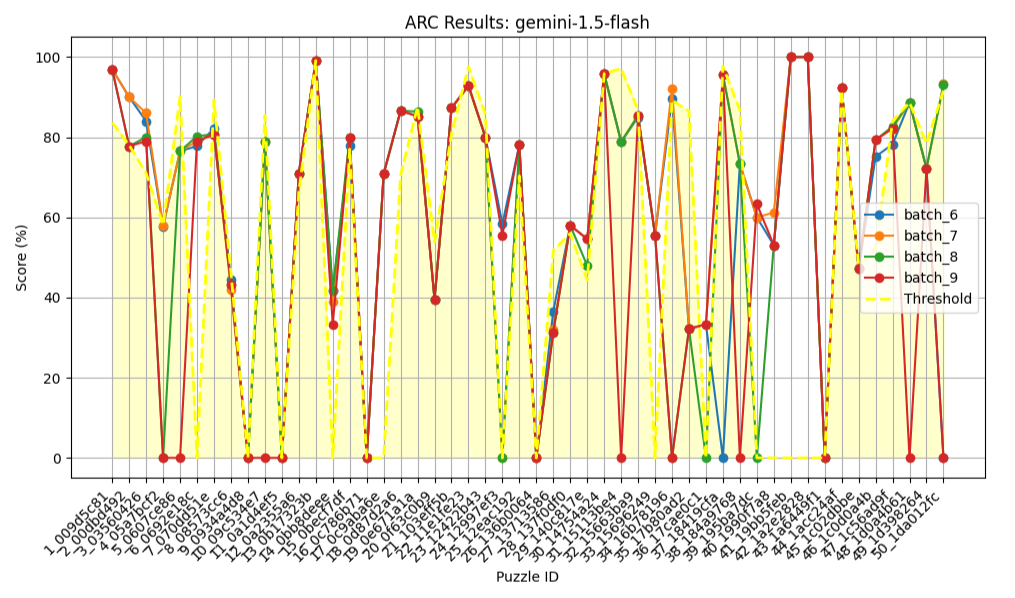
\includegraphics[width=0.99\linewidth, center]{gemini-1.5-flash.png}

\begin{table}[h]
    \centering
    \begin{tabular}{|c|c|c|c|c|c|}
        \hline
        Batch & Temp & Additional Examples & Total Attempted & Above Threshold & Solved 100\% \\ 
        \hline
        batch-0 & 1.65 & 0 & 47 & 21 & 0 (0.00\%)   \\ 
        batch-1 & 1.65 & 0+data & 50 & 21 & 1 (2.00\%)   \\ 
        batch-2 & 1.25 & 2+data & 48 & 20 & 1 (2.08\%)   \\ 
        batch-3 & 1.35 & 4+data & 45 & 21 & 0 (0.00\%)   \\ 
        \hline
    \end{tabular}
    \caption{ gemini-2.0-flash-thinking-exp-01-21 results }
    \label{tab:example}
\end{table}

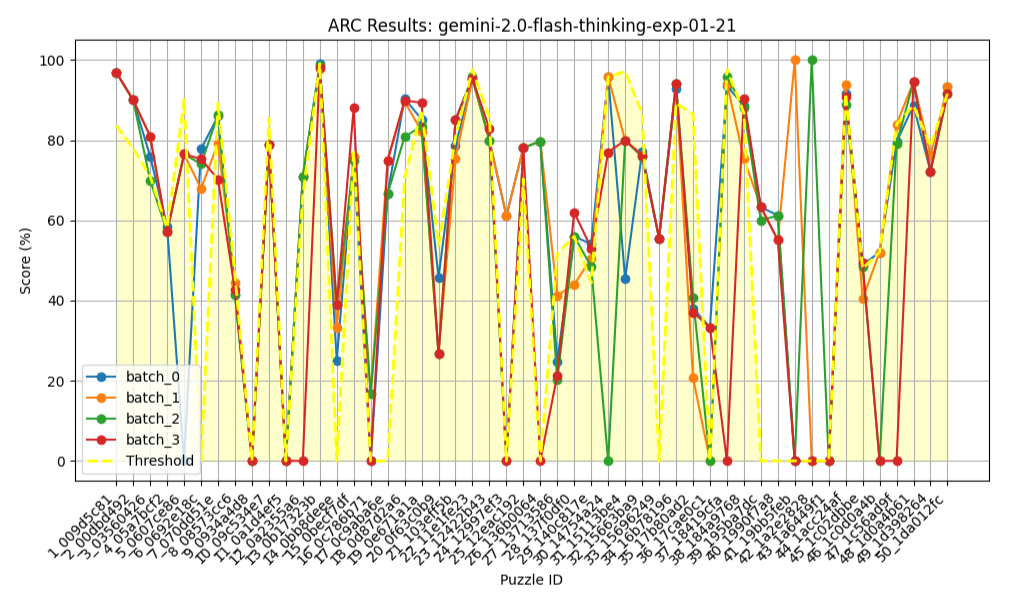
\includegraphics[width=0.99\linewidth, center]{gemini-2.0-flash-thinking-exp-01-21.png}

\vspace{2cm}

\textbf{Measuring True Intelligence: Challenges, Limitations, and a Proposal for AGI Criteria} \\
However, many challenges—such as achieving true reasoning, common sense, and ethical alignment—require breakthroughs that extend beyond merely scaling existing architectures. Until these advances are made, AI remains a powerful yet flawed tool that performs best under human oversight. Below is a list of key issues observed in current state-of-the-art LLMs:
\begin{itemize}
    \item Lack of true understanding/comprehension
    \item Lack of common sense
    \item Context limitations or shallow reasoning
    \item Resource intensity
    \item Lack of transparency (black box behavior)
    \item Vulnerability to adversarial attacks
    \item Hallucinations
\end{itemize}
Interestingly, none of these issues are self-identified by AI/LLMs; they are all diagnosed by humans—whether researchers, users, or auditors—through testing, analysis, or observation. Current AI/LLMs lack the self-awareness and introspection \cite{ref13} needed to autonomously recognize their own limitations. Although these systems can describe their flaws if prompted \cite{ref14}, this is based on training data (human-authored critiques) or web searches rather than genuine self-diagnosis. \\

As demonstrated in Table 1, top AI models have achieved remarkable scores on benchmarks related to common sense and basic science reasoning. Yet, despite these high scores, LLMs consistently falter when confronted with practical, novel scenarios. This discrepancy raises an important question: Can we accurately measure the core intelligence of a system when current AI benchmarks seem inadequate for this purpose? \\

At present, AI and LLMs have not independently invented any digital tool or function in the way that humans have created entirely novel and foundational innovations. However, human researchers have developed AI-generated enhancements and optimizations that significantly improve performance. In light of these observations, we propose a simple yet rigorous AGI criterion—one that tests an AI/LLM model's general intelligence and cannot be easily circumvented unless true AGI is achieved. \\

\begin{huge}
\textbf{AGI Criteria: Beyond Scaling LLMs}
\end{huge}
We have proposed a very simple 3 steps AGI criteria to check whether the current LLMs and future intelligent models hold the test of human level intelligence. An AI system can be considered Artificial General Intelligence (AGI) if it independently pass AGI Criteria without human intervention: \\ \\
\textbf{Analyze/Audit Itself} – The AI must recognize issues or limitations in its own body of code, reasoning, context and abstraction. \\
\textbf{Generate Solutions} – For a specific problem chosen by AI itself based on its priority It should be able to generate multiple possible ways to fix or improve itself. \\
\textbf{Implement and Repeat} – The AI must choose the best solution and implement it and repeat the process. \\

\textbf{Conditions}
AI Resources will remain constant during that process, initially limited amount of extra memory and resources should be provided to the AI system then it should remain constant then it should be upto the AI system to manage those resources like Humans do \\

\begin{huge}
\textbf{Design and Operational Implications} \\
\end{huge}
\textbf{Prioritization of Tasks:} \\
The AGI would need to learn which tasks are most critical and allocate resources accordingly. It might, for instance, reserve more memory for tasks that require deep introspection or learning, and less for routine operations. \\
\textbf{Trade-Offs and Decision-Making:} \\
Limited resources mean that the AI must sometimes make trade-offs. For example, a more resource-intensive self-analysis might be deferred in favor of immediate, less demanding tasks. This trade-off is similar to how humans decide between deep reflection and rapid decision-making based on available mental energy and time. \\
\textbf{Algorithmic Innovation:} \\
With a cap on resources, the AGI is pushed toward developing more efficient algorithms. This might lead to breakthroughs in how to compress information, optimize code, or structure reasoning in a way that minimizes overhead. \\
\textbf{Safety and Stability:} \\
Limiting resources can also serve as a safety mechanism. It prevents an AGI from overcommitting or making uncontrolled changes that might require external resources to manage—much like how our biological systems maintain homeostasis. \\

It is clear that \textbf{focusing exclusively on scaling LLMs is a fundamentally flawed approach to achieving General Intelligence}. The issue lies not merely in the scale of LLMs, but in the foundational limitations of the LLM approach. As demonstrated in several examples we have tested, including the three discussed earlier, ChatGPT and similar models continually fail to exhibit true reasoning or understanding beyond pattern recognition. For those interested, additional examples are available on our GitHub link \cite{ref8}, further proving that the current trajectory of LLM development is unlikely to fulfill the promise of AGI. Intelligence cannot be forced to emerge simply by tuning weights and biases, no matter how large the model's parameters or how extensive the training data. \\

LLMs, despite their impressive capabilities, are not progressing toward true intelligence—they excel at simulating responses but lack core attributes of intelligence, such as the ability to ask meaningful questions, innovate, or comprehend abstract concepts. \textbf{At best, LLMs can serve as one component within a broader intelligent system, but expecting them to form the sole foundation of AGI is misguided}. Intelligence is not about knowing everything; it is about confronting nuances with limited resources—qualities that cannot be engineered solely through data scaling and model optimization. To build a truly intelligent system, we need to fundamentally rethink our approach. \\ \\

\vspace{1cm}

\begin{huge}
\textbf{Conclusion}
\end{huge}

As demonstrated, current large language models (LLMs), while impressive in many respects, exhibit significant limitations that prevent them from attaining true intelligence. Their creativity is constrained by the scope of their training data, and they are fundamentally incapable of producing genuinely novel ideas. While they excel at pattern recognition, they lack essential qualities such as common sense, relational logic, and true understanding—core attributes of human intelligence. Rather than reasoning, they operate through memorized skill programs and statistical associations, which limits their ability to generalize or solve unfamiliar problems.

One of the most critical limitations is that LLMs approach all problems through their singular strength: \textbf{predicting the next word in a sequence}. Though this mechanism proves powerful for various tasks, it fails when confronted with multi-modal or abstract reasoning challenges. This is akin to deploying a highly specialized industrial robot designed to sort objects by color for a task requiring spatial reasoning or ethical judgment. The robot may perform flawlessly within its narrow scope but fails entirely when asked to adapt to contexts outside of its designed capabilities. Similarly, LLMs apply their language modeling paradigm indiscriminately—even to problems that require conceptual understanding or reasoning—exposing their lack of flexibility.

Moreover, a clear disparity exists between LLMs’ textual reasoning and their performance in visual or practical tasks, underscoring the absence of \textbf{integrated, cross-modal understanding}. While they may offer coherent textual descriptions, their inability to transfer this understanding to visual tasks—such as mechanical design—demonstrates a lack of grounded comprehension.

In summary, the current trajectory of LLM development relies heavily on augmenting their core strength rather than addressing foundational weaknesses. This patchwork approach may yield incremental improvements, but it is unlikely to result in true artificial general intelligence (AGI). \textbf{True intelligence demands the ability to question, abstract, and invent—capabilities that remain unique to human cognition}. Until LLMs transcend pattern recognition and demonstrate genuine reasoning, they will remain powerful yet fundamentally limited tools.

\vspace{1em}
\noindent
\textbf{Key Takeaways:}
\begin{itemize}
    \item LLMs are limited by their reliance on next-word prediction and lack true understanding or abstraction capabilities.
    \item They exhibit poor common-sense reasoning and fail at tasks requiring relational logic.
    \item Their textual and visual capabilities remain disconnected, revealing gaps in cross-modal reasoning.
    \item Pattern recognition alone is insufficient to achieve AGI.
    \item Human-like intelligence requires curiosity, creativity, and the ability to ask new questions—traits absent in LLMs.
\end{itemize}


\vspace{1cm}


\includegraphics[width=0.99\linewidth, center]{conclusion_image.png}

\vspace{1cm}

\begin{thebibliography}{14}  % The number indicates the widest reference label width

    \bibitem{ref1}
	Owain Evans, Lukas Berglund, Meg Tong, Max Kaufmann, et al. (2024). THE REVERSAL CURSE : LLMs TRAINED ON “A IS B” FAIL TO LEARN “B IS A”. arXiv:2309.12288v4.      
    \bibitem{ref2}
    Marianna Nezhurina, Lucia Cipolina-Kun, Mehdi Cherti, Jenia Jitsev, et al. (2024). Alice in Wonderland: Simple Tasks Showing Complete Reasoning Breakdown in State-Of-the-Art Large Language Models. arXiv:2406.02061v4.
    \bibitem{ref3}
    François Chollet. (2019). On the Measure of Intelligence. arXiv:1911.01547v2.
    \bibitem{ref4}
    Nouha Dziri, Ximing Lu, Melanie Sclar, Xiang Lorraine Li, Liwei Jiang, et al. (2023). Faith and Fate: Limits of Transformers on Compositionality. arXiv:2305.18654v3.
    \bibitem{ref5}
    Mengnan Du, Fengxiang He, Na Zou, Dacheng Tao, and Xia Hu. (2024). Shortcut Learning of Large Language Models in Natural Language Understanding. DOI:10.1145/3596490.
    \bibitem{ref6}
    Chen Ling, Xujiang Zhao, Jiaying Lu, Chengyuan Deng, Can Zheng, Junxiang Wang, et al. (2024). Domain Specialization as the Key to Make Large Language Models Disruptive: A Comprehensive Survey. arXiv:2305.18703v7.
    \bibitem{ref7}
	Karan Singhal, Shekoofeh Azizi, Tao Tu, S. Sara Mahdavi, Jason Wei, et al. (2022). Large Language Models Encode Clinical Knowledge. arXiv:2212.13138v1.
	\bibitem{ref8}
	Extra examples, Github Link: \url{https://github.com/ainumbat/ChatGPT4o_issues.git}
	\bibitem{ref9}
	François Chollet talk at AGI Conference, ARC Prize Youtube channel (2024). \url{https://www.youtube.com/watch?v=nL9jEy99Nh0&t=1450s}
	\bibitem{ref10}
	Xiang Lorraine Li, Adhiguna Kuncoro, Jordan Hoffmann, et al. (2022). A Systematic Investigation of Commonsense Knowledge in Large Language Models. arXiv:2111.00607v3.
	\bibitem{ref11}
	Jason Wei, Yi Tay, Rishi Bommasani, Colin Raffel, et al. (2022). Emergent Abilities of Large Language Models. arXiv:2206.07682v2 
    \bibitem{ref12}
	Jason Wei, Xuezhi Wang, Dale Schuurmans, et al. (2022). Chain-of-Thought Prompting Elicits Reasoning in Large Language Models. arXiv:2201.11903v6.     
	\bibitem{ref13}
	Zhangyue Yin, Qiushi Sun, Qipeng Guo, et al. (2023). Do Large Language Models Know What They Don’t Know? arXiv:2305.18153v2.
	\bibitem{ref14}
    Miles Turpin, Julian Michael, Ethan Perez, Samuel R. Bowman1, et al. (2023). Language Models Don’t Always Say What They Think: Unfaithful Explanations in Chain-of-Thought. arXiv:2305.04388v2. 
	\bibitem{ref15}    
    Georg Wenzel and Adam Jatowt. (2023). An Overview Of Temporal Commonsense Reasoning and Acquisition. arXiv:2308.00002v3.
    \bibitem{ref16}    
    François Chollet, Mike Knoop, Gregory Kamradt and Bryan Landers (2023). ARC Prize 2024: Technical Report. arXiv:2412.04604v2.
    \bibitem{ref17}    
    Jason Wei, Brian Ichter, Xuezhi Wang, Fei Xia, et al. (2023). Chain-of-Thought Prompting Elicits Reasoning
in Large Language Models. arXiv:2201.11903v6.
    \bibitem{ref18}    
    Jun Zhao, Jingqi Tong, Yurong Mou, et al. (2024). Exploring the Compositional Deficiency of Large Language Models in
Mathematical Reasoning Through Trap Problems. arXiv:2405.06680v4. 
    \bibitem{ref19}    
    Michael Timothy Bennett. (2024). Is Complexity an Illusion? arXiv:2404.07227v4.
    \bibitem{ref20}    
    Tyler A. Chang and Benjamin K. Bergen. (2023). Language Model Behavior: A Comprehensive Survey
    \bibitem{ref21}    
    Tom B. Brown, Benjamin Mann, Nick Ryder, Melanie Subbiah, et al. (2020). Language Models are Few-Shot Learners. arXiv:2005.14165v4 
    \bibitem{ref22}    
    Sourav Banerjee, Ayushi Agarwal and Saloni Singla. (2024). LLMs Will Always Hallucinate, and We Need to Live With This. arXiv:2409.05746v1.
    \bibitem{ref23}    
    Moritz Herrmann, Julian D. Lange, Katharina Eggensperger, et al. (2024). Position: Why We Must Rethink Empirical Research in Machine Learning. arXiv:2405.02200v2.
    \bibitem{ref24}    
    Zhaofeng Wuã, Linlu Qiuã, Alexis Ross, et al. (2024). Reasoning or Reciting? Exploring the Capabilities and Limitations of Language Models Through Counterfactual Tasks. arXiv:2307.02477v3.
    \bibitem{ref25}    
    Ekin Akyürek, Mehul Damani, Linlu Qiu, et al. (2024). The Surprising Effectiveness of Test-Time Training for Abstract Reasoning. arXiv:2411.07279v1.
\end{thebibliography}




































\end{document}